\begin{example}[A high-degree vertex can survive a peel phase]
\label{ex:algorithm-survivor-20260918}
This separate example illustrates the row contract used in
\cref{app:lem:successful-path-structure}, rather than specifying a
target--oracle pair.  Let $\DegreeCutoff=9$ and take the $65$ vertices
\[
 U=\{z\}\cup\{h_i:1\le i\le6\}
   \cup\{u_{i,j}:1\le i\le6,\ 1\le j\le9\}
   \cup\{s_1,s_2,s_3,s_4\},
\]
with edges
\[
 E=\{\{z,h_i\}:1\le i\le6\}
 \cup\{\{h_i,u_{i,j}\}:1\le i\le6,\ 1\le j\le9\}
 \cup\{\{z,s_j\}:1\le j\le4\}.
\]
At the history under consideration, take $\ResidualPositions=U$ and
$\ResidualForest=F=(U,E)$.
The center $z$ and all six hubs have degree $10$; all other vertices
are leaves.  Take the following row outputs, which obey the contract
\emph{exact at degree at most $d$, size at most $d$ elsewhere}:
\[
 \ScreenRow{z}=\ScreenRow{h_i}=\emptyset,\qquad
 \ScreenRow{u_{i,j}}=\{h_i\},\qquad
 \ScreenRow{s_j}=\{z\}.
\]
Computing the incoming counts, rather than reading a high-degree row's
size as its degree, gives
\begin{align*}
 \ClaimCount{z}&=4\le9/2, & \ClaimCount{h_i}&=9>9/2,\\
 \ClaimCount{u_{i,j}}&=\ClaimCount{s_j}=0,
 & \PeelSet&=\{h_1,\ldots,h_6\}.
\end{align*}
Thus $z$ is not peeled.  Before the commits its high-degree neighbors
are exactly $\{h_1,\ldots,h_6\}$, so their number is $6>9/2$, as required by
\eqref{app:eq:survivor-high-neighbors}.  After the six frozen singleton
commits in \AlgoBlockRef{peel}, its remaining neighbors are $\{s_1,\ldots,s_4\}$:
\begin{align*}
 d_{F[U\setminus\PeelSet]}(z)&=4,\\
 |\{v\in U:d_F(v)>9\}|&=7,\\
 |\{v\in U\setminus\PeelSet:d_{F[U\setminus\PeelSet]}(v)>9\}|&=0.
\end{align*}
The center survives as a vertex but ceases to be high-degree.
The $54$ hub leaves become isolated; none was committed in this phase.
\Cref{fig:algorithm-survivor-20260918} draws each of them separately.
\end{example}

\begin{figure}[H]
 \centering
 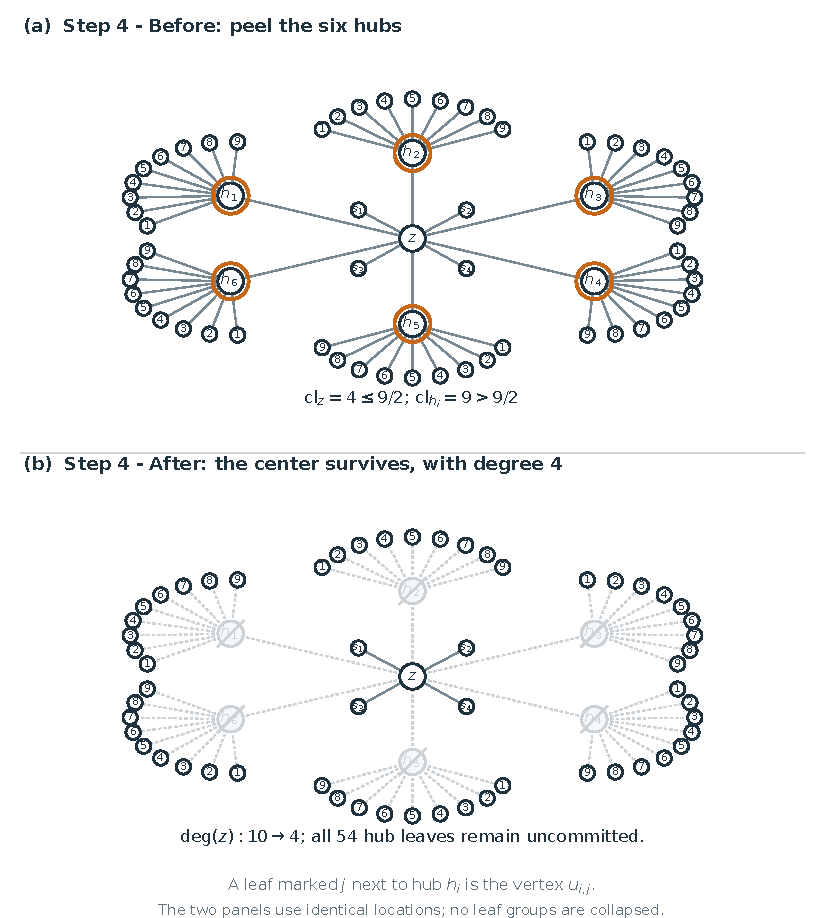
\includegraphics[width=\linewidth]{figures/algorithm_examples_2026-09-18/output/pdf/survivor_2026-09-18.pdf}
 \caption{The separate contraction example of
 \cref{ex:algorithm-survivor-20260918}. The six orange-ringed hubs are
 committed one at a time in \AlgoBlockRef{peel}, with no intervening screen or peel-set
 recomputation. Their $54$ leaves are drawn individually, not bundled.
 The unpeeled center $z$ changes from degree $10$ to degree $4$.
 The lower panel keeps the same locations and crosses out only the
 committed hubs.}
 \label{fig:algorithm-survivor-20260918}
\end{figure}
